\documentclass{cmn}
\usepackage{pgfplots}
\pgfplotsset{compat=1.18}
\usepgfplotslibrary{units}

\begin{document}
  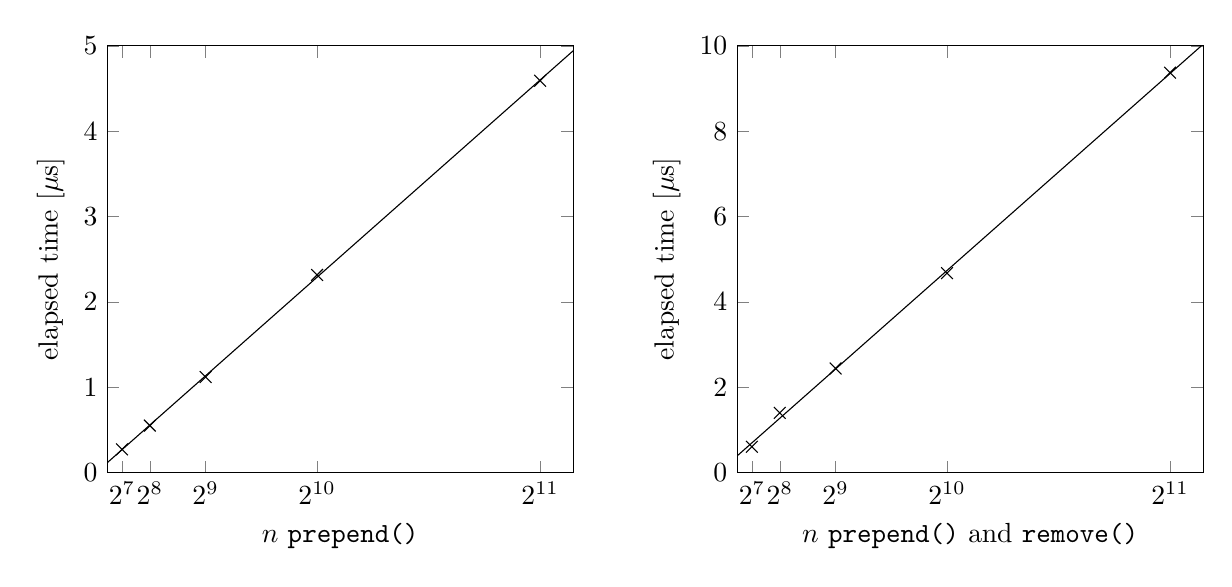
\begin{tikzpicture}
    \begin{scope}
      \begin{axis}[
        width=75mm,
        height=70mm,
        xlabel={$n$ \texttt{prepend()}},
        ylabel={elapsed time},
        xtick={128,256,512,1024,2048},
        xticklabels={$2^7$,$2^8$,$2^9$,$2^{10}$,$2^{11}$},
        ytick distance=1,
        y filter/.expression={0.001*y},
        use units,
        y unit=s,
        y unit prefix=\mu,
        xmin=60,
        xmax=2200,
        ymin=0,
        ymax=5,
      ]
        \addplot[only marks,mark=x,mark size=3pt] table [x=n,y=T]{
             n        T
           128  270.977
           256  549.189
           512 1118.513
          1024 2315.228
          2048 4590.432
        };
        \addplot[domain=60:2200] { 2.25645*x - 21.85058 };
      \end{axis}
    \end{scope}

    \begin{scope}[xshift=80mm]
      \begin{axis}[
        width=75mm,
        height=70mm,
        xlabel={$n$ \texttt{prepend()} and \texttt{remove()}},
        ylabel={elapsed time},
        xtick={128,256,512,1024,2048},
        xticklabels={$2^7$,$2^8$,$2^9$,$2^{10}$,$2^{11}$},
        ytick distance=2,
        y filter/.expression={0.001*y},
        use units,
        y unit=s,
        y unit prefix=\mu,
        xmin=60,
        xmax=2200,
        ymin=0,
        ymax=10,
      ]
        \addplot[only marks,mark=x,mark size=3pt] table [x=n,y=T]{
             n        T
           128  601.452
           256 1395.408
           512 2436.951
          1024 4670.832
          2048 9369.192
        };

        \addplot[domain=60:2200] { 4.50878*x + 116.59938 };
      \end{axis}
    \end{scope}
  \end{tikzpicture}
\end{document}
